% Overview of the infinite-order Chapman--Enskog convergence benchmark.
% Standalone: % Overview of the infinite-order Chapman--Enskog convergence benchmark.
% Standalone: % Overview of the infinite-order Chapman--Enskog convergence benchmark.
% Standalone: % Overview of the infinite-order Chapman--Enskog convergence benchmark.
% Standalone: \input{benchmark_chapman_enskog} from main.tex.
% Requires booktabs + graphicx; uses figures/fig_polyce_convergence.pdf and
% data/polyce_n2_convergence.tex. Produced by
% benchmark_polyatomic_chapman_enskog.m (re-plot: plot_polyce_convergence.m).
\section{Infinite-order Chapman--Enskog convergence}
\label{sec:ce}

The transport coefficients of Section~\ref{sec:transport} are those of the $17$-moment closure
\cite[eqs.~(35)--(39)]{Djordjic2023}: the shear viscosity $\mu=p/P_\sigma^{(0)}$ is a single ($1\times1$)
production coefficient, and the bulk viscosity and Prandtl number \eqref{eq:Pr} follow from the
$\ell=0$ and $\ell=1$ first-order blocks. This is the lowest Sonine order. Because our spectral operator
represents the linearized collision integral in a full Laguerre$\times$spherical-harmonic basis, we can
instead solve the Chapman--Enskog problem to \emph{arbitrary} order by directly inverting the growing
radial block -- the polyatomic counterpart of the infinite-order hard-sphere viscosity inversion of the
monatomic theory.

\paragraph{Method.}
At equilibrium the linearized operator $J=C(:,:,1)+C(:,1,:)$ block-diagonalizes by angular degree
$\ell$. For each transport coefficient we take the $\ell$-block (all internal modes $i=0,\dots,I_{\max}$
and radial modes $k=0,\dots,K_{\max}$, minus the conserved directions), Schur-reduce it onto the
first-order macroscopic moment(s), and read off the coefficient exactly as in \eqref{eq:Pr}. The
first-order truncation reproduces the $17$-moment values of Section~\ref{sec:transport} identically; each
extra radial order adds the corresponding higher-Sonine correction. For shear we report the correction
factor $f_\mu=\mu^{(K_{\max})}/\mu^{(1)}$; $K_{\max}$ is the radial (Sonine) truncation, with the internal
resolution held fixed at $I_{\max}$.

\paragraph{Validation.}
Two exact anchors confirm the inversion machinery before the extended model is switched on:
\begin{itemize}
\item \textbf{Maxwell ($\zeta=0$).} The basis diagonalizes the linearized operator (Wang--Chang--Uhlenbeck
spectrum), so $f_\mu\equiv1$ at every $K_{\max}$ to machine precision.
\item \textbf{Hard-sphere frozen ($\zeta=1,\ \omega=0$).} The elastic channel leaves internal energy a
spectator, so its $\ell=2$ block is the monatomic hard-sphere operator: $f_\mu$ recovers the exact
second-order fraction $205/202\approx1.014851$ and converges to the Pekeris infinite-order limit
$1.016034$ (to $\sim3\times10^{-5}$ at $K_{\max}=3$), matching classical kinetic theory
\cite{chapman:1970}.
\end{itemize}

\paragraph{Extended model (N$_2$).}
Table~\ref{tab:ce_n2} and Fig.~\ref{fig:ce} report the converged coefficients for N$_2$ at the extended-model
Table-4 parameters \cite[eq.~(43)]{Djordjic2023}. The Prandtl number is essentially resolution-independent
($0.723\!\to\!0.718$) and matches the experimental/fitted value $0.717$. The bulk/shear ratio, however,
exposes a two-part gap to the fitted target $\nu/\mu=0.730$:
\begin{itemize}
\item \textbf{Production-coefficient evaluation ($+0.12$, already at first order).} Djordji\'c et al.\ fit
the Table-4 parameters so that \emph{their} evaluation of the model \eqref{eq:Pr} equals experiment. The
production coefficients are not free parameters but computed collision integrals; evaluating the identical
kernel with our spectral quadrature gives $\nu/\mu=0.853$ already at first order. The discrepancy is
localized entirely to the bulk coefficient $P_\Pi^{(0)}$ -- the singular internal-energy relaxation
integral -- while the shear and heat-flux sectors agree to $<0.3\%$ (hence the matching $\Pr$). This is
consistent with the base-model finding of Section~\ref{sec:frozenpr} that our spectral quadrature evaluates
the internal-energy sector more accurately than the analytic/CAS reduction.
\item \textbf{Higher-order Sonine correction ($+0.06$).} Resolving the operator beyond the $17$-moment
closure raises $\nu/\mu$ from $0.853$ to a converged $0.912$; the shear factor rises to $f_\mu=1.0064$.
\end{itemize}
As a consistency check, the first-order values reproduce the independent E3 evaluation of
\texttt{benchmark\_dsmc\_extended} to four digits ($\nu/\mu=0.8535$, $\Pr=0.7187$ at padding $[16,16,8]$),
confirming the extraction. The absolute accuracy of the extended internal-energy exponents
$(\hat\eta,\hat\zeta)$ has not yet been cross-validated by an independent Monte-Carlo evaluation of
$P_\Pi^{(0)}$; the base kernel is anchored exactly (Section~\ref{sec:validation}).

\begin{table}[t]
\centering
\caption{N$_2$ transport coefficients: the experimental/fitted values of \cite{Djordjic2023}, our
first-order (17-moment) reproduction from the computed production coefficients, and the infinite-order
radial-block inversion converging in $K_{\max}$ ($I_{\max}=2$, $L_{\max}=2$).}
\label{tab:ce_n2}
\input{data/polyce_n2_convergence.tex}
\end{table}

\begin{figure}[t]
\centering
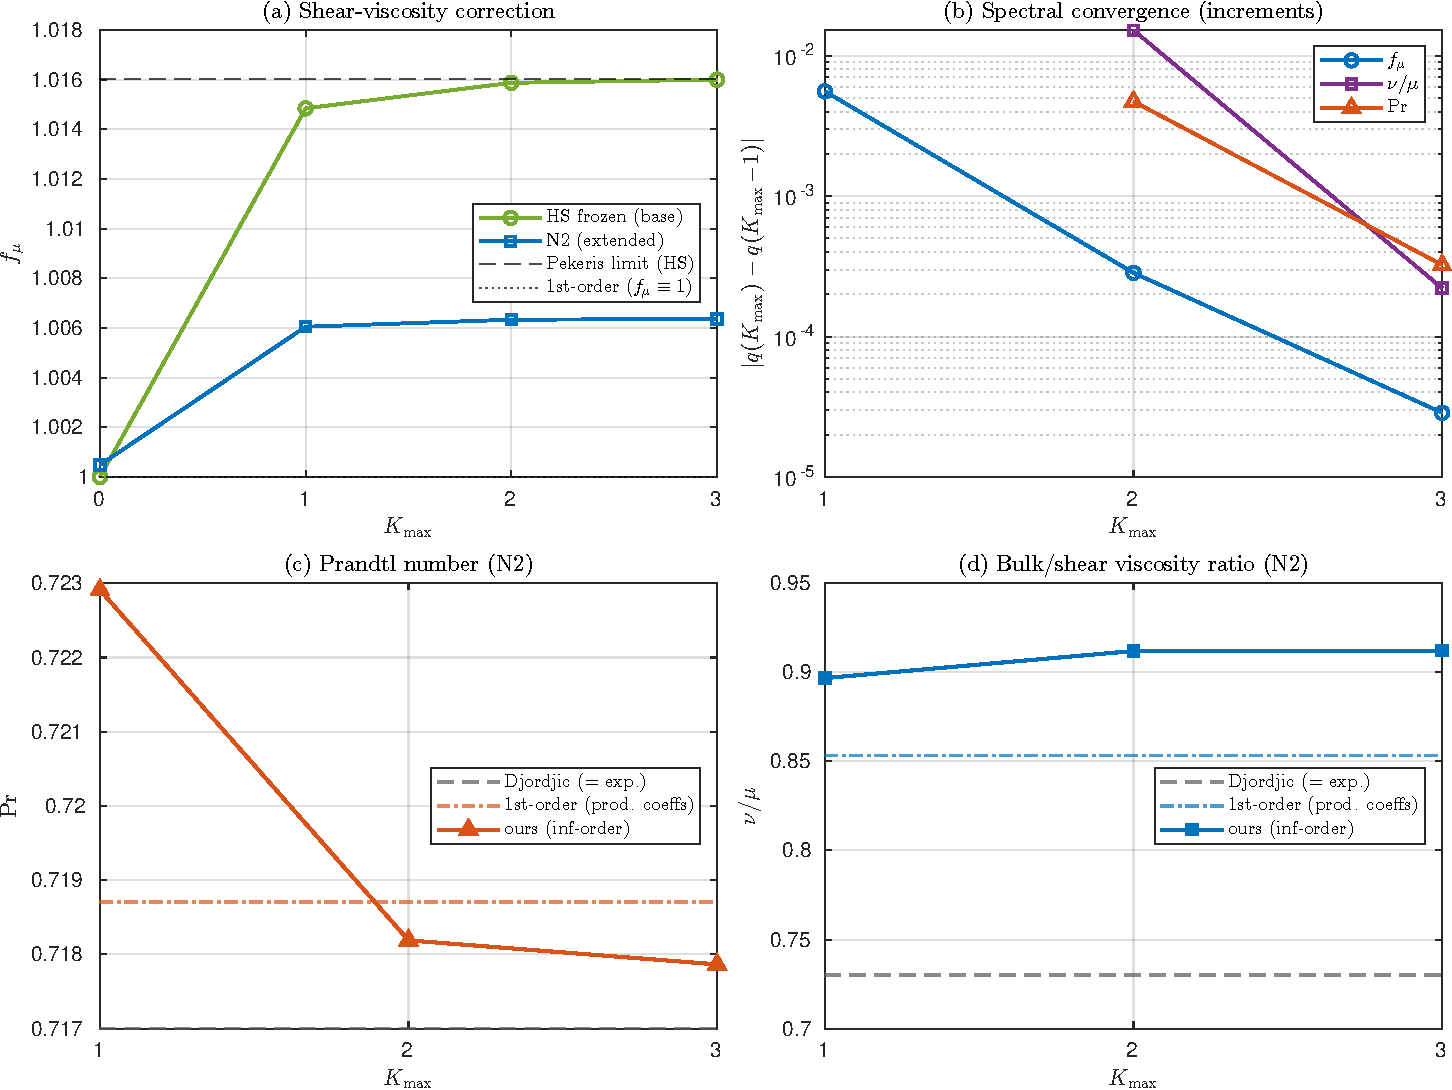
\includegraphics[width=0.9\textwidth]{figures/fig_polyce_convergence.pdf}
\caption{Infinite-order Chapman--Enskog convergence. (a) Shear correction $f_\mu$: the hard-sphere frozen
channel recovers the Pekeris limit (validation), while the extended N$_2$ model converges to $1.0064$.
(b) Spectral convergence (successive increments). (c)~Prandtl number and (d)~bulk/shear ratio for N$_2$:
our infinite-order values (solid) against Djordji\'c's fitted value (dashed) and our first-order
reproduction from the production coefficients (dash-dot). $\Pr$ matches; $\nu/\mu$ separates from the fitted
target by a production-coefficient evaluation difference plus a higher-order Sonine correction.}
\label{fig:ce}
\end{figure}
 from main.tex.
% Requires booktabs + graphicx; uses figures/fig_polyce_convergence.pdf and
% data/polyce_n2_convergence.tex. Produced by
% benchmark_polyatomic_chapman_enskog.m (re-plot: plot_polyce_convergence.m).
\section{Infinite-order Chapman--Enskog convergence}
\label{sec:ce}

The transport coefficients of Section~\ref{sec:transport} are those of the $17$-moment closure
\cite[eqs.~(35)--(39)]{Djordjic2023}: the shear viscosity $\mu=p/P_\sigma^{(0)}$ is a single ($1\times1$)
production coefficient, and the bulk viscosity and Prandtl number \eqref{eq:Pr} follow from the
$\ell=0$ and $\ell=1$ first-order blocks. This is the lowest Sonine order. Because our spectral operator
represents the linearized collision integral in a full Laguerre$\times$spherical-harmonic basis, we can
instead solve the Chapman--Enskog problem to \emph{arbitrary} order by directly inverting the growing
radial block -- the polyatomic counterpart of the infinite-order hard-sphere viscosity inversion of the
monatomic theory.

\paragraph{Method.}
At equilibrium the linearized operator $J=C(:,:,1)+C(:,1,:)$ block-diagonalizes by angular degree
$\ell$. For each transport coefficient we take the $\ell$-block (all internal modes $i=0,\dots,I_{\max}$
and radial modes $k=0,\dots,K_{\max}$, minus the conserved directions), Schur-reduce it onto the
first-order macroscopic moment(s), and read off the coefficient exactly as in \eqref{eq:Pr}. The
first-order truncation reproduces the $17$-moment values of Section~\ref{sec:transport} identically; each
extra radial order adds the corresponding higher-Sonine correction. For shear we report the correction
factor $f_\mu=\mu^{(K_{\max})}/\mu^{(1)}$; $K_{\max}$ is the radial (Sonine) truncation, with the internal
resolution held fixed at $I_{\max}$.

\paragraph{Validation.}
Two exact anchors confirm the inversion machinery before the extended model is switched on:
\begin{itemize}
\item \textbf{Maxwell ($\zeta=0$).} The basis diagonalizes the linearized operator (Wang--Chang--Uhlenbeck
spectrum), so $f_\mu\equiv1$ at every $K_{\max}$ to machine precision.
\item \textbf{Hard-sphere frozen ($\zeta=1,\ \omega=0$).} The elastic channel leaves internal energy a
spectator, so its $\ell=2$ block is the monatomic hard-sphere operator: $f_\mu$ recovers the exact
second-order fraction $205/202\approx1.014851$ and converges to the Pekeris infinite-order limit
$1.016034$ (to $\sim3\times10^{-5}$ at $K_{\max}=3$), matching classical kinetic theory
\cite{chapman:1970}.
\end{itemize}

\paragraph{Extended model (N$_2$).}
Table~\ref{tab:ce_n2} and Fig.~\ref{fig:ce} report the converged coefficients for N$_2$ at the extended-model
Table-4 parameters \cite[eq.~(43)]{Djordjic2023}. The Prandtl number is essentially resolution-independent
($0.723\!\to\!0.718$) and matches the experimental/fitted value $0.717$. The bulk/shear ratio, however,
exposes a two-part gap to the fitted target $\nu/\mu=0.730$:
\begin{itemize}
\item \textbf{Production-coefficient evaluation ($+0.12$, already at first order).} Djordji\'c et al.\ fit
the Table-4 parameters so that \emph{their} evaluation of the model \eqref{eq:Pr} equals experiment. The
production coefficients are not free parameters but computed collision integrals; evaluating the identical
kernel with our spectral quadrature gives $\nu/\mu=0.853$ already at first order. The discrepancy is
localized entirely to the bulk coefficient $P_\Pi^{(0)}$ -- the singular internal-energy relaxation
integral -- while the shear and heat-flux sectors agree to $<0.3\%$ (hence the matching $\Pr$). This is
consistent with the base-model finding of Section~\ref{sec:frozenpr} that our spectral quadrature evaluates
the internal-energy sector more accurately than the analytic/CAS reduction.
\item \textbf{Higher-order Sonine correction ($+0.06$).} Resolving the operator beyond the $17$-moment
closure raises $\nu/\mu$ from $0.853$ to a converged $0.912$; the shear factor rises to $f_\mu=1.0064$.
\end{itemize}
As a consistency check, the first-order values reproduce the independent E3 evaluation of
\texttt{benchmark\_dsmc\_extended} to four digits ($\nu/\mu=0.8535$, $\Pr=0.7187$ at padding $[16,16,8]$),
confirming the extraction. The absolute accuracy of the extended internal-energy exponents
$(\hat\eta,\hat\zeta)$ has not yet been cross-validated by an independent Monte-Carlo evaluation of
$P_\Pi^{(0)}$; the base kernel is anchored exactly (Section~\ref{sec:validation}).

\begin{table}[t]
\centering
\caption{N$_2$ transport coefficients: the experimental/fitted values of \cite{Djordjic2023}, our
first-order (17-moment) reproduction from the computed production coefficients, and the infinite-order
radial-block inversion converging in $K_{\max}$ ($I_{\max}=2$, $L_{\max}=2$).}
\label{tab:ce_n2}
% Auto-generated by benchmark_polyatomic_chapman_enskog.m
\begin{tabular}{lccc}
\toprule
 & $f_\mu$ & $\nu/\mu$ & $\mathrm{Pr}$ \\
\midrule
Experiment (Djordji\'c) & --- & 0.730 & 0.717 \\
1st-order (prod. coeffs) & 1.0000 & 0.8533 & 0.7187 \\
\midrule
$K_{\max}=0$ & 1.0005 & --- & --- \\
$K_{\max}=1$ & 1.0061 & 0.8968 & 0.7229 \\
$K_{\max}=2$ & 1.0063 & 0.9120 & 0.7182 \\
$K_{\max}=3$ & 1.0064 & 0.9122 & 0.7179 \\
\bottomrule
\end{tabular}

\end{table}

\begin{figure}[t]
\centering
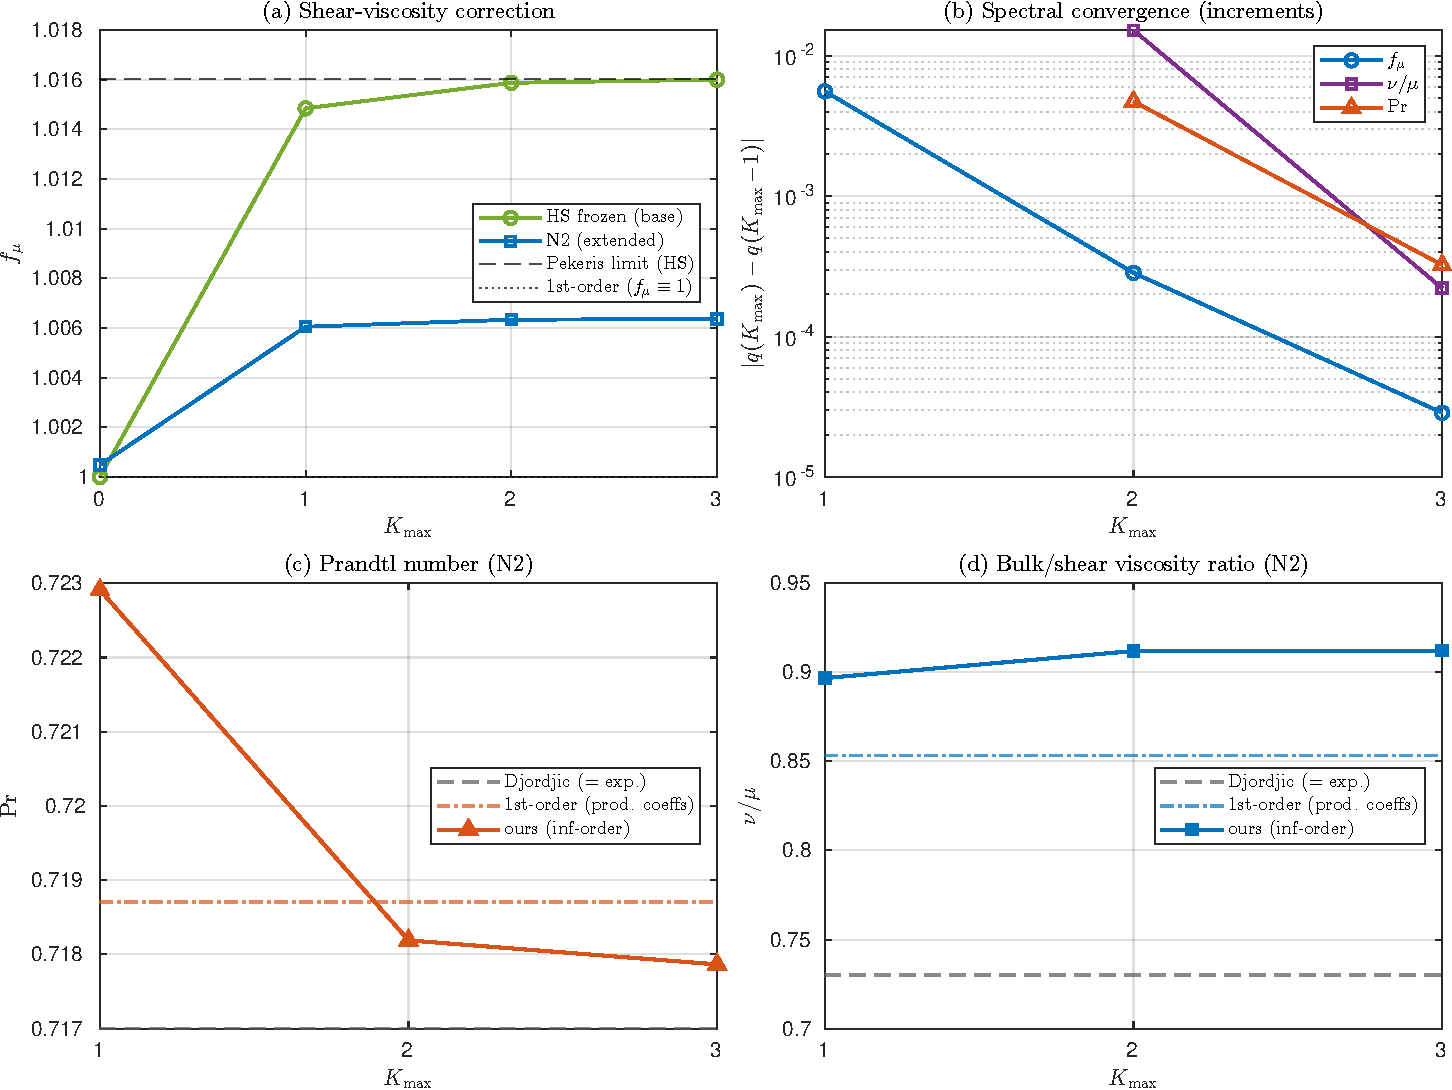
\includegraphics[width=0.9\textwidth]{figures/fig_polyce_convergence.pdf}
\caption{Infinite-order Chapman--Enskog convergence. (a) Shear correction $f_\mu$: the hard-sphere frozen
channel recovers the Pekeris limit (validation), while the extended N$_2$ model converges to $1.0064$.
(b) Spectral convergence (successive increments). (c)~Prandtl number and (d)~bulk/shear ratio for N$_2$:
our infinite-order values (solid) against Djordji\'c's fitted value (dashed) and our first-order
reproduction from the production coefficients (dash-dot). $\Pr$ matches; $\nu/\mu$ separates from the fitted
target by a production-coefficient evaluation difference plus a higher-order Sonine correction.}
\label{fig:ce}
\end{figure}
 from main.tex.
% Requires booktabs + graphicx; uses figures/fig_polyce_convergence.pdf and
% data/polyce_n2_convergence.tex. Produced by
% benchmark_polyatomic_chapman_enskog.m (re-plot: plot_polyce_convergence.m).
\section{Infinite-order Chapman--Enskog convergence}
\label{sec:ce}

The transport coefficients of Section~\ref{sec:transport} are those of the $17$-moment closure
\cite[eqs.~(35)--(39)]{Djordjic2023}: the shear viscosity $\mu=p/P_\sigma^{(0)}$ is a single ($1\times1$)
production coefficient, and the bulk viscosity and Prandtl number \eqref{eq:Pr} follow from the
$\ell=0$ and $\ell=1$ first-order blocks. This is the lowest Sonine order. Because our spectral operator
represents the linearized collision integral in a full Laguerre$\times$spherical-harmonic basis, we can
instead solve the Chapman--Enskog problem to \emph{arbitrary} order by directly inverting the growing
radial block -- the polyatomic counterpart of the infinite-order hard-sphere viscosity inversion of the
monatomic theory.

\paragraph{Method.}
At equilibrium the linearized operator $J=C(:,:,1)+C(:,1,:)$ block-diagonalizes by angular degree
$\ell$. For each transport coefficient we take the $\ell$-block (all internal modes $i=0,\dots,I_{\max}$
and radial modes $k=0,\dots,K_{\max}$, minus the conserved directions), Schur-reduce it onto the
first-order macroscopic moment(s), and read off the coefficient exactly as in \eqref{eq:Pr}. The
first-order truncation reproduces the $17$-moment values of Section~\ref{sec:transport} identically; each
extra radial order adds the corresponding higher-Sonine correction. For shear we report the correction
factor $f_\mu=\mu^{(K_{\max})}/\mu^{(1)}$; $K_{\max}$ is the radial (Sonine) truncation, with the internal
resolution held fixed at $I_{\max}$.

\paragraph{Validation.}
Two exact anchors confirm the inversion machinery before the extended model is switched on:
\begin{itemize}
\item \textbf{Maxwell ($\zeta=0$).} The basis diagonalizes the linearized operator (Wang--Chang--Uhlenbeck
spectrum), so $f_\mu\equiv1$ at every $K_{\max}$ to machine precision.
\item \textbf{Hard-sphere frozen ($\zeta=1,\ \omega=0$).} The elastic channel leaves internal energy a
spectator, so its $\ell=2$ block is the monatomic hard-sphere operator: $f_\mu$ recovers the exact
second-order fraction $205/202\approx1.014851$ and converges to the Pekeris infinite-order limit
$1.016034$ (to $\sim3\times10^{-5}$ at $K_{\max}=3$), matching classical kinetic theory
\cite{chapman:1970}.
\end{itemize}

\paragraph{Extended model (N$_2$).}
Table~\ref{tab:ce_n2} and Fig.~\ref{fig:ce} report the converged coefficients for N$_2$ at the extended-model
Table-4 parameters \cite[eq.~(43)]{Djordjic2023}. The Prandtl number is essentially resolution-independent
($0.723\!\to\!0.718$) and matches the experimental/fitted value $0.717$. The bulk/shear ratio, however,
exposes a two-part gap to the fitted target $\nu/\mu=0.730$:
\begin{itemize}
\item \textbf{Production-coefficient evaluation ($+0.12$, already at first order).} Djordji\'c et al.\ fit
the Table-4 parameters so that \emph{their} evaluation of the model \eqref{eq:Pr} equals experiment. The
production coefficients are not free parameters but computed collision integrals; evaluating the identical
kernel with our spectral quadrature gives $\nu/\mu=0.853$ already at first order. The discrepancy is
localized entirely to the bulk coefficient $P_\Pi^{(0)}$ -- the singular internal-energy relaxation
integral -- while the shear and heat-flux sectors agree to $<0.3\%$ (hence the matching $\Pr$). This is
consistent with the base-model finding of Section~\ref{sec:frozenpr} that our spectral quadrature evaluates
the internal-energy sector more accurately than the analytic/CAS reduction.
\item \textbf{Higher-order Sonine correction ($+0.06$).} Resolving the operator beyond the $17$-moment
closure raises $\nu/\mu$ from $0.853$ to a converged $0.912$; the shear factor rises to $f_\mu=1.0064$.
\end{itemize}
As a consistency check, the first-order values reproduce the independent E3 evaluation of
\texttt{benchmark\_dsmc\_extended} to four digits ($\nu/\mu=0.8535$, $\Pr=0.7187$ at padding $[16,16,8]$),
confirming the extraction. The absolute accuracy of the extended internal-energy exponents
$(\hat\eta,\hat\zeta)$ has not yet been cross-validated by an independent Monte-Carlo evaluation of
$P_\Pi^{(0)}$; the base kernel is anchored exactly (Section~\ref{sec:validation}).

\begin{table}[t]
\centering
\caption{N$_2$ transport coefficients: the experimental/fitted values of \cite{Djordjic2023}, our
first-order (17-moment) reproduction from the computed production coefficients, and the infinite-order
radial-block inversion converging in $K_{\max}$ ($I_{\max}=2$, $L_{\max}=2$).}
\label{tab:ce_n2}
% Auto-generated by benchmark_polyatomic_chapman_enskog.m
\begin{tabular}{lccc}
\toprule
 & $f_\mu$ & $\nu/\mu$ & $\mathrm{Pr}$ \\
\midrule
Experiment (Djordji\'c) & --- & 0.730 & 0.717 \\
1st-order (prod. coeffs) & 1.0000 & 0.8533 & 0.7187 \\
\midrule
$K_{\max}=0$ & 1.0005 & --- & --- \\
$K_{\max}=1$ & 1.0061 & 0.8968 & 0.7229 \\
$K_{\max}=2$ & 1.0063 & 0.9120 & 0.7182 \\
$K_{\max}=3$ & 1.0064 & 0.9122 & 0.7179 \\
\bottomrule
\end{tabular}

\end{table}

\begin{figure}[t]
\centering
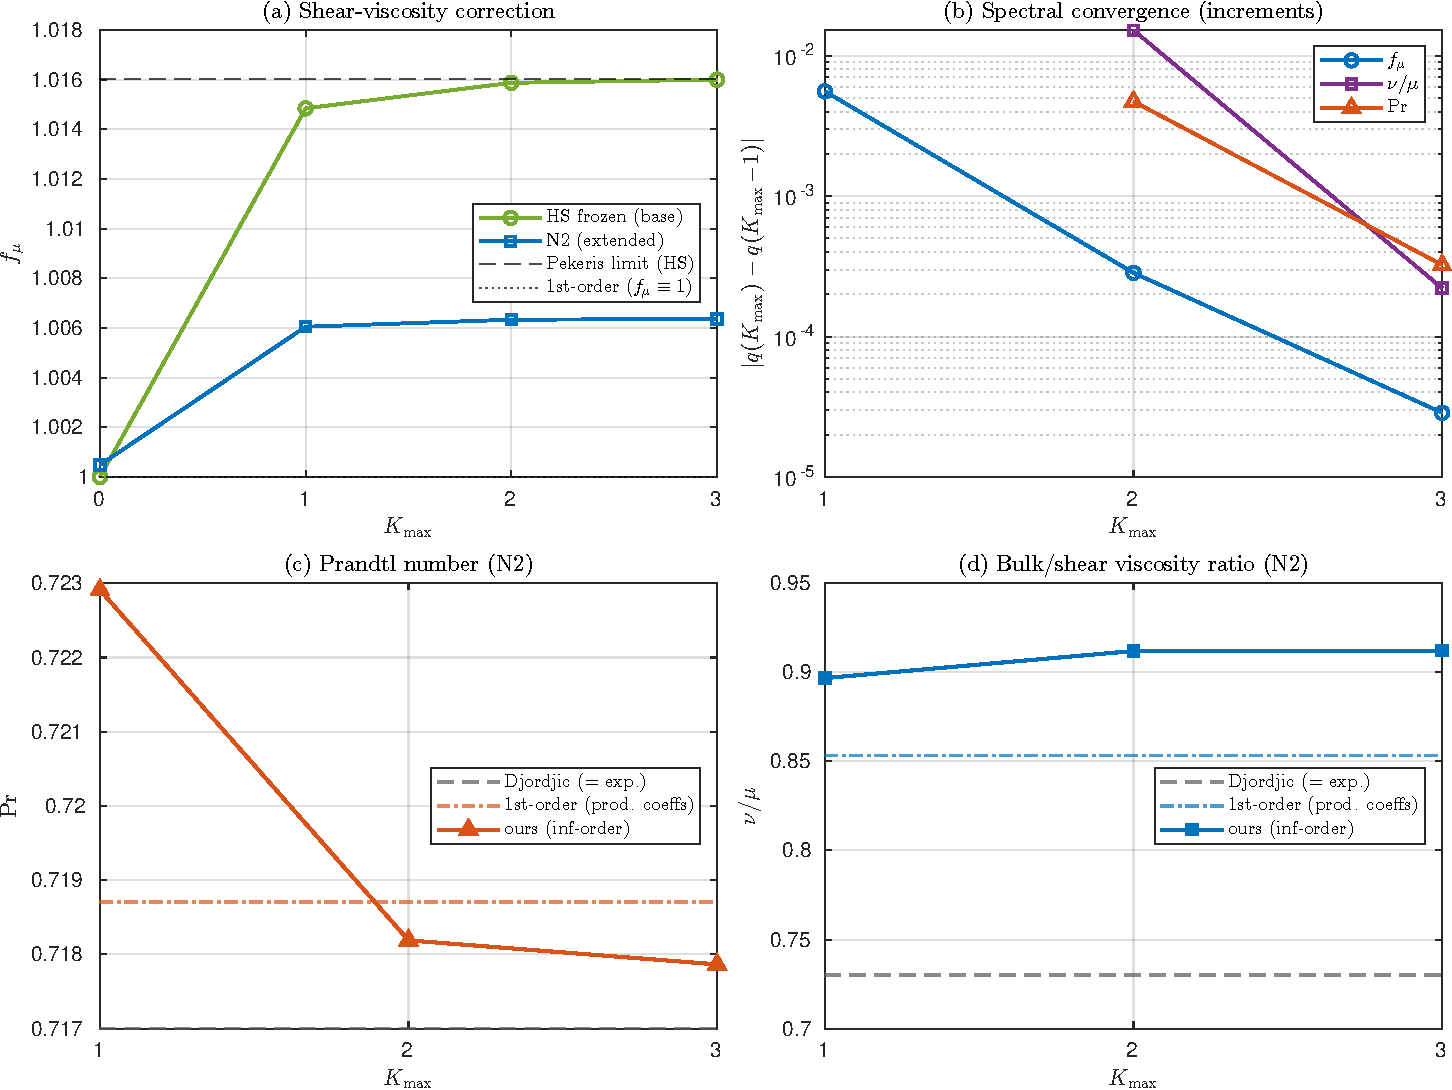
\includegraphics[width=0.9\textwidth]{figures/fig_polyce_convergence.pdf}
\caption{Infinite-order Chapman--Enskog convergence. (a) Shear correction $f_\mu$: the hard-sphere frozen
channel recovers the Pekeris limit (validation), while the extended N$_2$ model converges to $1.0064$.
(b) Spectral convergence (successive increments). (c)~Prandtl number and (d)~bulk/shear ratio for N$_2$:
our infinite-order values (solid) against Djordji\'c's fitted value (dashed) and our first-order
reproduction from the production coefficients (dash-dot). $\Pr$ matches; $\nu/\mu$ separates from the fitted
target by a production-coefficient evaluation difference plus a higher-order Sonine correction.}
\label{fig:ce}
\end{figure}
 from main.tex.
% Requires booktabs + graphicx; uses figures/fig_polyce_convergence.pdf and
% data/polyce_n2_convergence.tex. Produced by
% benchmark_polyatomic_chapman_enskog.m (re-plot: plot_polyce_convergence.m).
\section{Infinite-order Chapman--Enskog convergence}
\label{sec:ce}

The transport coefficients of Section~\ref{sec:transport} are those of the $17$-moment closure
\cite[eqs.~(35)--(39)]{Djordjic2023}: the shear viscosity $\mu=p/P_\sigma^{(0)}$ is a single ($1\times1$)
production coefficient, and the bulk viscosity and Prandtl number \eqref{eq:Pr} follow from the
$\ell=0$ and $\ell=1$ first-order blocks. This is the lowest Sonine order. Because our spectral operator
represents the linearized collision integral in a full Laguerre$\times$spherical-harmonic basis, we can
instead solve the Chapman--Enskog problem to \emph{arbitrary} order by directly inverting the growing
radial block -- the polyatomic counterpart of the infinite-order hard-sphere viscosity inversion of the
monatomic theory.

\paragraph{Method.}
At equilibrium the linearized operator $J=C(:,:,1)+C(:,1,:)$ block-diagonalizes by angular degree
$\ell$. For each transport coefficient we take the $\ell$-block (all internal modes $i=0,\dots,I_{\max}$
and radial modes $k=0,\dots,K_{\max}$, minus the conserved directions), Schur-reduce it onto the
first-order macroscopic moment(s), and read off the coefficient exactly as in \eqref{eq:Pr}. The
first-order truncation reproduces the $17$-moment values of Section~\ref{sec:transport} identically; each
extra radial order adds the corresponding higher-Sonine correction. For shear we report the correction
factor $f_\mu=\mu^{(K_{\max})}/\mu^{(1)}$; $K_{\max}$ is the radial (Sonine) truncation, with the internal
resolution held fixed at $I_{\max}$.

\paragraph{Validation.}
Two exact anchors confirm the inversion machinery before the extended model is switched on:
\begin{itemize}
\item \textbf{Maxwell ($\zeta=0$).} The basis diagonalizes the linearized operator (Wang--Chang--Uhlenbeck
spectrum), so $f_\mu\equiv1$ at every $K_{\max}$ to machine precision.
\item \textbf{Hard-sphere frozen ($\zeta=1,\ \omega=0$).} The elastic channel leaves internal energy a
spectator, so its $\ell=2$ block is the monatomic hard-sphere operator: $f_\mu$ recovers the exact
second-order fraction $205/202\approx1.014851$ and converges to the Pekeris infinite-order limit
$1.016034$ (to $\sim3\times10^{-5}$ at $K_{\max}=3$), matching classical kinetic theory
\cite{chapman:1970}.
\end{itemize}

\paragraph{Extended model (N$_2$).}
Table~\ref{tab:ce_n2} and Fig.~\ref{fig:ce} report the converged coefficients for N$_2$ at the extended-model
Table-4 parameters \cite[eq.~(43)]{Djordjic2023}. The Prandtl number is essentially resolution-independent
($0.723\!\to\!0.718$) and matches the experimental/fitted value $0.717$. The bulk/shear ratio, however,
exposes a two-part gap to the fitted target $\nu/\mu=0.730$:
\begin{itemize}
\item \textbf{Production-coefficient evaluation ($+0.12$, already at first order).} Djordji\'c et al.\ fit
the Table-4 parameters so that \emph{their} evaluation of the model \eqref{eq:Pr} equals experiment. The
production coefficients are not free parameters but computed collision integrals; evaluating the identical
kernel with our spectral quadrature gives $\nu/\mu=0.853$ already at first order. The discrepancy is
localized entirely to the bulk coefficient $P_\Pi^{(0)}$ -- the singular internal-energy relaxation
integral -- while the shear and heat-flux sectors agree to $<0.3\%$ (hence the matching $\Pr$). This is
consistent with the base-model finding of Section~\ref{sec:frozenpr} that our spectral quadrature evaluates
the internal-energy sector more accurately than the analytic/CAS reduction.
\item \textbf{Higher-order Sonine correction ($+0.06$).} Resolving the operator beyond the $17$-moment
closure raises $\nu/\mu$ from $0.853$ to a converged $0.912$; the shear factor rises to $f_\mu=1.0064$.
\end{itemize}
As a consistency check, the first-order values reproduce the independent E3 evaluation of
\texttt{benchmark\_dsmc\_extended} to four digits ($\nu/\mu=0.8535$, $\Pr=0.7187$ at padding $[16,16,8]$),
confirming the extraction. The absolute accuracy of the extended internal-energy exponents
$(\hat\eta,\hat\zeta)$ has not yet been cross-validated by an independent Monte-Carlo evaluation of
$P_\Pi^{(0)}$; the base kernel is anchored exactly (Section~\ref{sec:validation}).

\begin{table}[t]
\centering
\caption{N$_2$ transport coefficients: the experimental/fitted values of \cite{Djordjic2023}, our
first-order (17-moment) reproduction from the computed production coefficients, and the infinite-order
radial-block inversion converging in $K_{\max}$ ($I_{\max}=2$, $L_{\max}=2$).}
\label{tab:ce_n2}
% Auto-generated by benchmark_polyatomic_chapman_enskog.m
\begin{tabular}{lccc}
\toprule
 & $f_\mu$ & $\nu/\mu$ & $\mathrm{Pr}$ \\
\midrule
Experiment (Djordji\'c) & --- & 0.730 & 0.717 \\
1st-order (prod. coeffs) & 1.0000 & 0.8533 & 0.7187 \\
\midrule
$K_{\max}=0$ & 1.0005 & --- & --- \\
$K_{\max}=1$ & 1.0061 & 0.8968 & 0.7229 \\
$K_{\max}=2$ & 1.0063 & 0.9120 & 0.7182 \\
$K_{\max}=3$ & 1.0064 & 0.9122 & 0.7179 \\
\bottomrule
\end{tabular}

\end{table}

\begin{figure}[t]
\centering
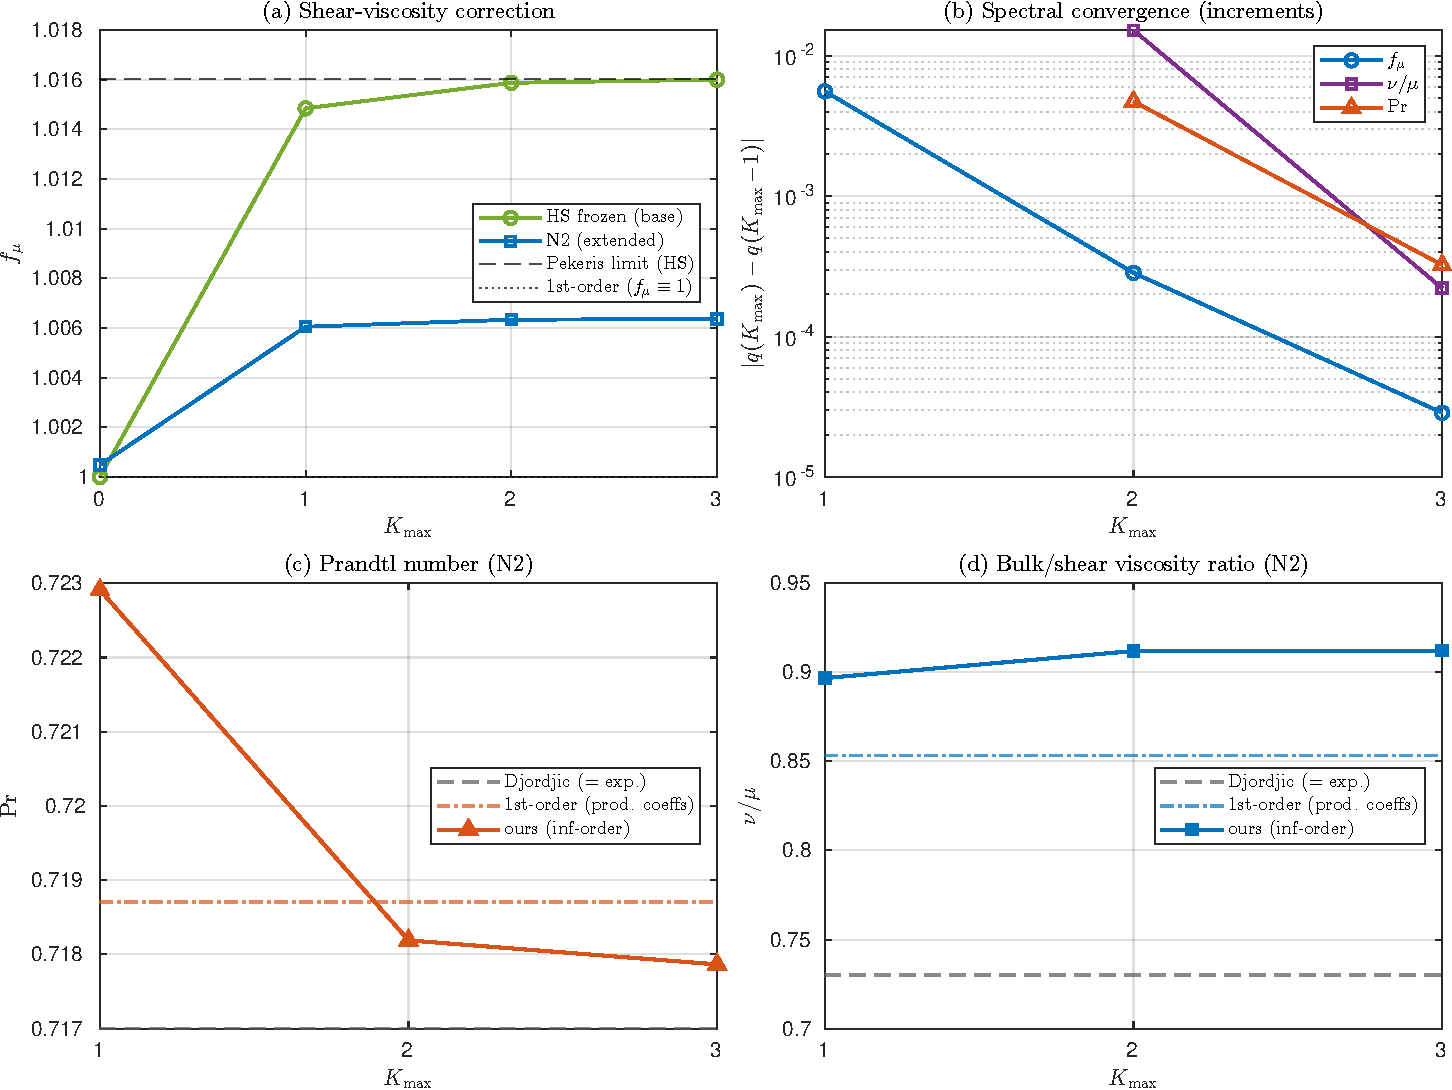
\includegraphics[width=0.9\textwidth]{figures/fig_polyce_convergence.pdf}
\caption{Infinite-order Chapman--Enskog convergence. (a) Shear correction $f_\mu$: the hard-sphere frozen
channel recovers the Pekeris limit (validation), while the extended N$_2$ model converges to $1.0064$.
(b) Spectral convergence (successive increments). (c)~Prandtl number and (d)~bulk/shear ratio for N$_2$:
our infinite-order values (solid) against Djordji\'c's fitted value (dashed) and our first-order
reproduction from the production coefficients (dash-dot). $\Pr$ matches; $\nu/\mu$ separates from the fitted
target by a production-coefficient evaluation difference plus a higher-order Sonine correction.}
\label{fig:ce}
\end{figure}
